% Options for packages loaded elsewhere
% Options for packages loaded elsewhere
\PassOptionsToPackage{unicode}{hyperref}
\PassOptionsToPackage{hyphens}{url}
\PassOptionsToPackage{dvipsnames,svgnames,x11names}{xcolor}
%
\documentclass[
  spanish,
  11pt,
  a4paper,
  DIV=11,
  numbers=noendperiod]{scrartcl}
\usepackage{xcolor}
\usepackage[margin=2.5cm]{geometry}
\usepackage{amsmath,amssymb}
\setcounter{secnumdepth}{5}
\usepackage{iftex}
\ifPDFTeX
  \usepackage[T1]{fontenc}
  \usepackage[utf8]{inputenc}
  \usepackage{textcomp} % provide euro and other symbols
\else % if luatex or xetex
  \usepackage{unicode-math} % this also loads fontspec
  \defaultfontfeatures{Scale=MatchLowercase}
  \defaultfontfeatures[\rmfamily]{Ligatures=TeX,Scale=1}
\fi
\usepackage{lmodern}
\ifPDFTeX\else
  % xetex/luatex font selection
  \setmainfont[]{Times New Roman}
\fi
% Use upquote if available, for straight quotes in verbatim environments
\IfFileExists{upquote.sty}{\usepackage{upquote}}{}
\IfFileExists{microtype.sty}{% use microtype if available
  \usepackage[]{microtype}
  \UseMicrotypeSet[protrusion]{basicmath} % disable protrusion for tt fonts
}{}
\makeatletter
\@ifundefined{KOMAClassName}{% if non-KOMA class
  \IfFileExists{parskip.sty}{%
    \usepackage{parskip}
  }{% else
    \setlength{\parindent}{0pt}
    \setlength{\parskip}{6pt plus 2pt minus 1pt}}
}{% if KOMA class
  \KOMAoptions{parskip=half}}
\makeatother
% Make \paragraph and \subparagraph free-standing
\makeatletter
\ifx\paragraph\undefined\else
  \let\oldparagraph\paragraph
  \renewcommand{\paragraph}{
    \@ifstar
      \xxxParagraphStar
      \xxxParagraphNoStar
  }
  \newcommand{\xxxParagraphStar}[1]{\oldparagraph*{#1}\mbox{}}
  \newcommand{\xxxParagraphNoStar}[1]{\oldparagraph{#1}\mbox{}}
\fi
\ifx\subparagraph\undefined\else
  \let\oldsubparagraph\subparagraph
  \renewcommand{\subparagraph}{
    \@ifstar
      \xxxSubParagraphStar
      \xxxSubParagraphNoStar
  }
  \newcommand{\xxxSubParagraphStar}[1]{\oldsubparagraph*{#1}\mbox{}}
  \newcommand{\xxxSubParagraphNoStar}[1]{\oldsubparagraph{#1}\mbox{}}
\fi
\makeatother

\usepackage{color}
\usepackage{fancyvrb}
\newcommand{\VerbBar}{|}
\newcommand{\VERB}{\Verb[commandchars=\\\{\}]}
\DefineVerbatimEnvironment{Highlighting}{Verbatim}{commandchars=\\\{\}}
% Add ',fontsize=\small' for more characters per line
\usepackage{framed}
\definecolor{shadecolor}{RGB}{241,243,245}
\newenvironment{Shaded}{\begin{snugshade}}{\end{snugshade}}
\newcommand{\AlertTok}[1]{\textcolor[rgb]{0.68,0.00,0.00}{#1}}
\newcommand{\AnnotationTok}[1]{\textcolor[rgb]{0.37,0.37,0.37}{#1}}
\newcommand{\AttributeTok}[1]{\textcolor[rgb]{0.40,0.45,0.13}{#1}}
\newcommand{\BaseNTok}[1]{\textcolor[rgb]{0.68,0.00,0.00}{#1}}
\newcommand{\BuiltInTok}[1]{\textcolor[rgb]{0.00,0.23,0.31}{#1}}
\newcommand{\CharTok}[1]{\textcolor[rgb]{0.13,0.47,0.30}{#1}}
\newcommand{\CommentTok}[1]{\textcolor[rgb]{0.37,0.37,0.37}{#1}}
\newcommand{\CommentVarTok}[1]{\textcolor[rgb]{0.37,0.37,0.37}{\textit{#1}}}
\newcommand{\ConstantTok}[1]{\textcolor[rgb]{0.56,0.35,0.01}{#1}}
\newcommand{\ControlFlowTok}[1]{\textcolor[rgb]{0.00,0.23,0.31}{\textbf{#1}}}
\newcommand{\DataTypeTok}[1]{\textcolor[rgb]{0.68,0.00,0.00}{#1}}
\newcommand{\DecValTok}[1]{\textcolor[rgb]{0.68,0.00,0.00}{#1}}
\newcommand{\DocumentationTok}[1]{\textcolor[rgb]{0.37,0.37,0.37}{\textit{#1}}}
\newcommand{\ErrorTok}[1]{\textcolor[rgb]{0.68,0.00,0.00}{#1}}
\newcommand{\ExtensionTok}[1]{\textcolor[rgb]{0.00,0.23,0.31}{#1}}
\newcommand{\FloatTok}[1]{\textcolor[rgb]{0.68,0.00,0.00}{#1}}
\newcommand{\FunctionTok}[1]{\textcolor[rgb]{0.28,0.35,0.67}{#1}}
\newcommand{\ImportTok}[1]{\textcolor[rgb]{0.00,0.46,0.62}{#1}}
\newcommand{\InformationTok}[1]{\textcolor[rgb]{0.37,0.37,0.37}{#1}}
\newcommand{\KeywordTok}[1]{\textcolor[rgb]{0.00,0.23,0.31}{\textbf{#1}}}
\newcommand{\NormalTok}[1]{\textcolor[rgb]{0.00,0.23,0.31}{#1}}
\newcommand{\OperatorTok}[1]{\textcolor[rgb]{0.37,0.37,0.37}{#1}}
\newcommand{\OtherTok}[1]{\textcolor[rgb]{0.00,0.23,0.31}{#1}}
\newcommand{\PreprocessorTok}[1]{\textcolor[rgb]{0.68,0.00,0.00}{#1}}
\newcommand{\RegionMarkerTok}[1]{\textcolor[rgb]{0.00,0.23,0.31}{#1}}
\newcommand{\SpecialCharTok}[1]{\textcolor[rgb]{0.37,0.37,0.37}{#1}}
\newcommand{\SpecialStringTok}[1]{\textcolor[rgb]{0.13,0.47,0.30}{#1}}
\newcommand{\StringTok}[1]{\textcolor[rgb]{0.13,0.47,0.30}{#1}}
\newcommand{\VariableTok}[1]{\textcolor[rgb]{0.07,0.07,0.07}{#1}}
\newcommand{\VerbatimStringTok}[1]{\textcolor[rgb]{0.13,0.47,0.30}{#1}}
\newcommand{\WarningTok}[1]{\textcolor[rgb]{0.37,0.37,0.37}{\textit{#1}}}

\usepackage{longtable,booktabs,array}
\usepackage{calc} % for calculating minipage widths
% Correct order of tables after \paragraph or \subparagraph
\usepackage{etoolbox}
\makeatletter
\patchcmd\longtable{\par}{\if@noskipsec\mbox{}\fi\par}{}{}
\makeatother
% Allow footnotes in longtable head/foot
\IfFileExists{footnotehyper.sty}{\usepackage{footnotehyper}}{\usepackage{footnote}}
\makesavenoteenv{longtable}
\usepackage{graphicx}
\makeatletter
\newsavebox\pandoc@box
\newcommand*\pandocbounded[1]{% scales image to fit in text height/width
  \sbox\pandoc@box{#1}%
  \Gscale@div\@tempa{\textheight}{\dimexpr\ht\pandoc@box+\dp\pandoc@box\relax}%
  \Gscale@div\@tempb{\linewidth}{\wd\pandoc@box}%
  \ifdim\@tempb\p@<\@tempa\p@\let\@tempa\@tempb\fi% select the smaller of both
  \ifdim\@tempa\p@<\p@\scalebox{\@tempa}{\usebox\pandoc@box}%
  \else\usebox{\pandoc@box}%
  \fi%
}
% Set default figure placement to htbp
\def\fps@figure{htbp}
\makeatother



\ifLuaTeX
\usepackage[bidi=basic]{babel}
\else
\usepackage[bidi=default]{babel}
\fi
\ifPDFTeX
\else
\babelfont{rm}[]{Times New Roman}
\fi
% get rid of language-specific shorthands (see #6817):
\let\LanguageShortHands\languageshorthands
\def\languageshorthands#1{}


\setlength{\emergencystretch}{3em} % prevent overfull lines

\providecommand{\tightlist}{%
  \setlength{\itemsep}{0pt}\setlength{\parskip}{0pt}}



 


\usepackage{booktabs}
\usepackage{longtable}
\usepackage{array}
\usepackage{multirow}
\usepackage{wrapfig}
\usepackage{float}
\usepackage{colortbl}
\usepackage{pdflscape}
\usepackage{tabu}
\usepackage{threeparttable}
\usepackage{threeparttablex}
\usepackage[normalem]{ulem}
\usepackage{makecell}
\usepackage{xcolor}
\usepackage[hidelinks]{hyperref}
\KOMAoption{captions}{tableheading}
\makeatletter
\@ifpackageloaded{caption}{}{\usepackage{caption}}
\AtBeginDocument{%
\ifdefined\contentsname
  \renewcommand*\contentsname{Tabla de contenidos}
\else
  \newcommand\contentsname{Tabla de contenidos}
\fi
\ifdefined\listfigurename
  \renewcommand*\listfigurename{Listado de Figuras}
\else
  \newcommand\listfigurename{Listado de Figuras}
\fi
\ifdefined\listtablename
  \renewcommand*\listtablename{Listado de Tablas}
\else
  \newcommand\listtablename{Listado de Tablas}
\fi
\ifdefined\figurename
  \renewcommand*\figurename{Figura}
\else
  \newcommand\figurename{Figura}
\fi
\ifdefined\tablename
  \renewcommand*\tablename{Tabla}
\else
  \newcommand\tablename{Tabla}
\fi
}
\@ifpackageloaded{float}{}{\usepackage{float}}
\floatstyle{ruled}
\@ifundefined{c@chapter}{\newfloat{codelisting}{h}{lop}}{\newfloat{codelisting}{h}{lop}[chapter]}
\floatname{codelisting}{Listado}
\newcommand*\listoflistings{\listof{codelisting}{Listado de Listados}}
\makeatother
\makeatletter
\makeatother
\makeatletter
\@ifpackageloaded{caption}{}{\usepackage{caption}}
\@ifpackageloaded{subcaption}{}{\usepackage{subcaption}}
\makeatother
\usepackage{bookmark}
\IfFileExists{xurl.sty}{\usepackage{xurl}}{} % add URL line breaks if available
\urlstyle{same}
\hypersetup{
  pdftitle={MANOVA-perMANOVA},
  pdfauthor={Santos G},
  pdflang={es},
  colorlinks=true,
  linkcolor={blue},
  filecolor={Maroon},
  citecolor={Blue},
  urlcolor={Blue},
  pdfcreator={LaTeX via pandoc}}


\title{MANOVA-perMANOVA}
\author{Santos G}
\date{}
\begin{document}
\maketitle

\renewcommand*\contentsname{Tabla de contenidos}
{
\hypersetup{linkcolor=}
\setcounter{tocdepth}{2}
\tableofcontents
}

\section{Contexto del proyecto}\label{contexto-del-proyecto}

Se evalúan supuestos (homogeneidad de matrices de covarianza, normalidad
multivariada y univariada, outliers multivariados), se ajusta el MANOVA
(test de Pillai) sobre dos variables transformadas (log10 de sépalos), y
se realizan comparaciones post-hoc por variable. Además, se utiliza
perMANOVA, prueba usada cuando no se cumplen los supuestos de normalidad
multivariada u homogeneidad de varianzas-covarianzas. En lugar de
basarse en distribuciones teóricas, esta prueba evalúa las diferencias
entre grupos mediante permutaciones de las distancias entre
observaciones, lo que la hace más robusta ante desviaciones de los
supuestos clásicos.

\section{Carga de librerías}\label{carga-de-libreruxedas}

\begin{Shaded}
\begin{Highlighting}[numbers=left,,]
\FunctionTok{library}\NormalTok{(tidyverse)      }\CommentTok{\# Conjunto de paquetes para el análisis de datos}
\FunctionTok{library}\NormalTok{(MVN)            }\CommentTok{\# Pruebas de normalidad multivariada}
\FunctionTok{library}\NormalTok{(biotools)       }\CommentTok{\# Box\textquotesingle{}s M test para homogeneidad }
\FunctionTok{library}\NormalTok{(rstatix)        }\CommentTok{\# Funciones para análisis comunes }
\FunctionTok{library}\NormalTok{(car)            }\CommentTok{\# Herramientas para análisis estadístico complementario}
\FunctionTok{library}\NormalTok{(emmeans)        }\CommentTok{\# Comparaciones post{-}hoc}
\FunctionTok{library}\NormalTok{(knitr)          }\CommentTok{\# Generación de reportes dinámicos en R Markdown}
\FunctionTok{library}\NormalTok{(kableExtra)     }\CommentTok{\# Mejora la presentación de tablas}
\FunctionTok{library}\NormalTok{(reshape2)       }\CommentTok{\# Reestructuración de datos}
\FunctionTok{library}\NormalTok{(vegan)          }\CommentTok{\# Análisis multivariante de comunidades ecológicas}
\FunctionTok{library}\NormalTok{(RVAideMemoire)  }\CommentTok{\# PERMANOVA y análisis no paramétricos}
\end{Highlighting}
\end{Shaded}

\section{Preparación MANOVA}\label{preparaciuxf3n-manova}

\begin{Shaded}
\begin{Highlighting}[numbers=left,,]
\CommentTok{\# Datos}
\FunctionTok{data}\NormalTok{(}\StringTok{"iris"}\NormalTok{)}
\NormalTok{df\_manova }\OtherTok{\textless{}{-}}\NormalTok{ iris }\SpecialCharTok{\%\textgreater{}\%} \FunctionTok{as\_tibble}\NormalTok{()}

\CommentTok{\# Transformaciones propuestas: log10 de Sepal.Length y Sepal.Width}
\NormalTok{df\_manova }\OtherTok{\textless{}{-}}\NormalTok{ df\_manova }\SpecialCharTok{\%\textgreater{}\%}
  \FunctionTok{mutate}\NormalTok{(}
    \AttributeTok{Sepal.LengthLog10 =} \FunctionTok{log10}\NormalTok{(Sepal.Length),}
    \AttributeTok{Sepal.WidthLog10  =} \FunctionTok{log10}\NormalTok{(Sepal.Width)}
\NormalTok{  )}
\end{Highlighting}
\end{Shaded}

\section{Verificación de supuestos}\label{verificaciuxf3n-de-supuestos}

\begin{Shaded}
\begin{Highlighting}[numbers=left,,]
\CommentTok{\# Función segura para extraer resultados MVN::mvn en formato consistente}
\NormalTok{mvn\_by\_group }\OtherTok{\textless{}{-}} \ControlFlowTok{function}\NormalTok{(data, group\_var, vars) \{}
\NormalTok{  groups }\OtherTok{\textless{}{-}} \FunctionTok{unique}\NormalTok{(data[[group\_var]])}
\NormalTok{  out }\OtherTok{\textless{}{-}} \FunctionTok{map\_dfr}\NormalTok{(groups, }\ControlFlowTok{function}\NormalTok{(g) \{}
\NormalTok{    sub }\OtherTok{\textless{}{-}}\NormalTok{ data }\SpecialCharTok{\%\textgreater{}\%} \FunctionTok{filter}\NormalTok{((}\SpecialCharTok{!!}\FunctionTok{sym}\NormalTok{(group\_var)) }\SpecialCharTok{==}\NormalTok{ g) }\SpecialCharTok{\%\textgreater{}\%} \FunctionTok{select}\NormalTok{(}\FunctionTok{all\_of}\NormalTok{(vars))}
    \CommentTok{\# usamos mvn con mvn\_test = "mardia", univariate\_test = "AD" }
\NormalTok{    res }\OtherTok{\textless{}{-}} \FunctionTok{tryCatch}\NormalTok{(}
\NormalTok{      MVN}\SpecialCharTok{::}\FunctionTok{mvn}\NormalTok{(sub, }\AttributeTok{mvn\_test =} \StringTok{"mardia"}\NormalTok{, }\AttributeTok{univariate\_test =} \StringTok{"AD"}\NormalTok{, }
               \AttributeTok{descriptives =} \ConstantTok{FALSE}\NormalTok{, }\AttributeTok{tidy =} \ConstantTok{TRUE}\NormalTok{),}
      \AttributeTok{error =} \ControlFlowTok{function}\NormalTok{(e) }\FunctionTok{return}\NormalTok{(}\ConstantTok{NULL}\NormalTok{)}
\NormalTok{    )}
    \ControlFlowTok{if}\NormalTok{ (}\FunctionTok{is.null}\NormalTok{(res)) \{}
      \FunctionTok{tibble}\NormalTok{(}\AttributeTok{Especie =} \FunctionTok{as.character}\NormalTok{(g), }\AttributeTok{Test =} \ConstantTok{NA}\NormalTok{, }\AttributeTok{Statistic =} \ConstantTok{NA}\NormalTok{, }
             \AttributeTok{p.value =} \ConstantTok{NA}\NormalTok{, }\AttributeTok{MVN =} \ConstantTok{NA}\NormalTok{)}
\NormalTok{    \} }\ControlFlowTok{else}\NormalTok{ \{}
\NormalTok{      df }\OtherTok{\textless{}{-}}\NormalTok{ res}\SpecialCharTok{$}\NormalTok{multivariate\_normality}
      \FunctionTok{tibble}\NormalTok{(}
        \AttributeTok{Especie =} \FunctionTok{as.character}\NormalTok{(g),}
        \AttributeTok{Test =}\NormalTok{ df}\SpecialCharTok{$}\NormalTok{Test,}
        \AttributeTok{Statistic =} \FunctionTok{round}\NormalTok{(}\FunctionTok{as.numeric}\NormalTok{(df}\SpecialCharTok{$}\NormalTok{Statistic), }\DecValTok{3}\NormalTok{),}
        \AttributeTok{p.value =} \FunctionTok{ifelse}\NormalTok{(df}\SpecialCharTok{$}\NormalTok{p.value }\SpecialCharTok{\textless{}} \FloatTok{0.001}\NormalTok{, }\StringTok{"\textless{} 0.001"}\NormalTok{, }
                         \FunctionTok{round}\NormalTok{(}\FunctionTok{as.numeric}\NormalTok{(df}\SpecialCharTok{$}\NormalTok{p.value), }\DecValTok{3}\NormalTok{)),}
        \AttributeTok{MVN =}\NormalTok{ df}\SpecialCharTok{$}\NormalTok{MVN}
\NormalTok{      )}
\NormalTok{    \}}
\NormalTok{  \})}
\NormalTok{  out}
\NormalTok{\}}

\NormalTok{vars\_manova }\OtherTok{\textless{}{-}} \FunctionTok{c}\NormalTok{(}\StringTok{"Sepal.LengthLog10"}\NormalTok{, }\StringTok{"Sepal.WidthLog10"}\NormalTok{)}
\NormalTok{lda\_mvn\_mult\_tbl }\OtherTok{\textless{}{-}} \FunctionTok{mvn\_by\_group}\NormalTok{(df\_manova, }\StringTok{"Species"}\NormalTok{, vars\_manova)}
\NormalTok{knitr}\SpecialCharTok{::}\FunctionTok{kable}\NormalTok{(lda\_mvn\_mult\_tbl)}
\end{Highlighting}
\end{Shaded}

\begin{longtable}[]{@{}llrrl@{}}

\caption{\label{tbl-manova-mvn-mult}Normalidad multivariada por especie
(test de Mardia)}

\tabularnewline

\toprule\noalign{}
Especie & Test & Statistic & p.value & MVN \\
\midrule\noalign{}
\endhead
\bottomrule\noalign{}
\endlastfoot
setosa & Mardia Skewness & 6.928 & 0.140 & ✓ Normal \\
setosa & Mardia Kurtosis & 1.483 & 0.138 & ✓ Normal \\
versicolor & Mardia Skewness & 4.206 & 0.379 & ✓ Normal \\
versicolor & Mardia Kurtosis & -0.516 & 0.606 & ✓ Normal \\
virginica & Mardia Skewness & 4.033 & 0.402 & ✓ Normal \\
virginica & Mardia Kurtosis & 0.651 & 0.515 & ✓ Normal \\

\end{longtable}

La Tabla~\ref{tbl-manova-mvn-mult} muestra los resultados de la prueba
de normalidad multivariada de Mardia aplicada a cada una de las especies
del conjunto \emph{iris}.

En todos los casos \emph{setosa}, \emph{versicolor} y \emph{virginica}
los valores de p asociados tanto a la asimetría como a la curtosis son
superiores a 0.05, indicando que no existen desviaciones significativas
respecto a la normalidad multivariada.

Por lo tanto, los datos pueden considerarse consistentes con este
supuesto, lo que respalda la validez del uso de técnicas multivariadas
como el análisis multivariado de la varianza (MANOVA) en este conjunto.

\begin{Shaded}
\begin{Highlighting}[numbers=left,,]
\CommentTok{\# Extraer univar de MVN::mvn por especie (AD)}
\NormalTok{mvn\_univar\_by\_group }\OtherTok{\textless{}{-}} \ControlFlowTok{function}\NormalTok{(data, group\_var, vars) \{}
\NormalTok{  groups }\OtherTok{\textless{}{-}} \FunctionTok{unique}\NormalTok{(data[[group\_var]])}
  \FunctionTok{map\_dfr}\NormalTok{(groups, }\ControlFlowTok{function}\NormalTok{(g) \{}
\NormalTok{    sub }\OtherTok{\textless{}{-}}\NormalTok{ data }\SpecialCharTok{\%\textgreater{}\%} \FunctionTok{filter}\NormalTok{((}\SpecialCharTok{!!}\FunctionTok{sym}\NormalTok{(group\_var)) }\SpecialCharTok{==}\NormalTok{ g) }\SpecialCharTok{\%\textgreater{}\%} \FunctionTok{select}\NormalTok{(}\FunctionTok{all\_of}\NormalTok{(vars))}
\NormalTok{    res }\OtherTok{\textless{}{-}} \FunctionTok{tryCatch}\NormalTok{(}
\NormalTok{      MVN}\SpecialCharTok{::}\FunctionTok{mvn}\NormalTok{(sub, }\AttributeTok{mvn\_test =} \StringTok{"mardia"}\NormalTok{, }\AttributeTok{univariate\_test =} \StringTok{"AD"}\NormalTok{, }
               \AttributeTok{descriptives =} \ConstantTok{FALSE}\NormalTok{, }\AttributeTok{tidy =} \ConstantTok{TRUE}\NormalTok{),}
      \AttributeTok{error =} \ControlFlowTok{function}\NormalTok{(e) }\FunctionTok{return}\NormalTok{(}\ConstantTok{NULL}\NormalTok{)}
\NormalTok{    )}
    \ControlFlowTok{if}\NormalTok{ (}\FunctionTok{is.null}\NormalTok{(res)) \{}
      \FunctionTok{tibble}\NormalTok{(}\AttributeTok{Especie =} \FunctionTok{as.character}\NormalTok{(g), }\AttributeTok{Test =} \ConstantTok{NA}\NormalTok{, }\AttributeTok{Variable =} \ConstantTok{NA}\NormalTok{, }
             \AttributeTok{Statistic =} \ConstantTok{NA}\NormalTok{, }\AttributeTok{p.value =} \ConstantTok{NA}\NormalTok{, }\AttributeTok{Normality =} \ConstantTok{NA}\NormalTok{)}
\NormalTok{    \} }\ControlFlowTok{else}\NormalTok{ \{}
\NormalTok{      df }\OtherTok{\textless{}{-}}\NormalTok{ res}\SpecialCharTok{$}\NormalTok{univariate\_normality }\SpecialCharTok{\%\textgreater{}\%} \FunctionTok{as\_tibble}\NormalTok{()}
\NormalTok{      df }\SpecialCharTok{\%\textgreater{}\%}
        \FunctionTok{mutate}\NormalTok{(}\AttributeTok{Especie =} \FunctionTok{as.character}\NormalTok{(g),}
               \AttributeTok{p.value =} \FunctionTok{ifelse}\NormalTok{(p.value }\SpecialCharTok{\textless{}} \FloatTok{0.001}\NormalTok{, }\StringTok{"\textless{} 0.001"}\NormalTok{, }
                                \FunctionTok{round}\NormalTok{(}\FunctionTok{as.numeric}\NormalTok{(p.value), }\DecValTok{3}\NormalTok{))) }\SpecialCharTok{\%\textgreater{}\%}
        \FunctionTok{select}\NormalTok{(Especie, Test, Variable, Statistic, }
\NormalTok{               p.value, Normality)}
\NormalTok{    \}}
\NormalTok{  \})}
\NormalTok{\}}

\NormalTok{lda\_mvn\_uni\_tbl }\OtherTok{\textless{}{-}} \FunctionTok{mvn\_univar\_by\_group}\NormalTok{(df\_manova, }\StringTok{"Species"}\NormalTok{, vars\_manova)}
\NormalTok{knitr}\SpecialCharTok{::}\FunctionTok{kable}\NormalTok{(lda\_mvn\_uni\_tbl)}
\end{Highlighting}
\end{Shaded}

\begin{longtable}[]{@{}
  >{\raggedright\arraybackslash}p{(\linewidth - 10\tabcolsep) * \real{0.1429}}
  >{\raggedright\arraybackslash}p{(\linewidth - 10\tabcolsep) * \real{0.2208}}
  >{\raggedright\arraybackslash}p{(\linewidth - 10\tabcolsep) * \real{0.2338}}
  >{\raggedleft\arraybackslash}p{(\linewidth - 10\tabcolsep) * \real{0.1299}}
  >{\raggedleft\arraybackslash}p{(\linewidth - 10\tabcolsep) * \real{0.1039}}
  >{\raggedright\arraybackslash}p{(\linewidth - 10\tabcolsep) * \real{0.1688}}@{}}

\caption{\label{tbl-manova-mvn-uni}Normalidad univariada por especie
(Anderson--Darling)}

\tabularnewline

\toprule\noalign{}
\begin{minipage}[b]{\linewidth}\raggedright
Especie
\end{minipage} & \begin{minipage}[b]{\linewidth}\raggedright
Test
\end{minipage} & \begin{minipage}[b]{\linewidth}\raggedright
Variable
\end{minipage} & \begin{minipage}[b]{\linewidth}\raggedleft
Statistic
\end{minipage} & \begin{minipage}[b]{\linewidth}\raggedleft
p.value
\end{minipage} & \begin{minipage}[b]{\linewidth}\raggedright
Normality
\end{minipage} \\
\midrule\noalign{}
\endhead
\bottomrule\noalign{}
\endlastfoot
setosa & Anderson-Darling & Sepal.LengthLog10 & 0.411 & 0.329 & ✓
Normal \\
setosa & Anderson-Darling & Sepal.WidthLog10 & 0.485 & 0.217 & ✓
Normal \\
versicolor & Anderson-Darling & Sepal.LengthLog10 & 0.320 & 0.523 & ✓
Normal \\
versicolor & Anderson-Darling & Sepal.WidthLog10 & 0.805 & 0.035 & ✗ Not
normal \\
virginica & Anderson-Darling & Sepal.LengthLog10 & 0.425 & 0.305 & ✓
Normal \\
virginica & Anderson-Darling & Sepal.WidthLog10 & 0.554 & 0.145 & ✓
Normal \\

\end{longtable}

La Tabla~\ref{tbl-manova-mvn-uni} presenta los resultados de la prueba
de normalidad univariada de Anderson--Darling para las variables
transformadas \emph{Sepal.LengthLog10} y \emph{Sepal.WidthLog10} en cada
especie del conjunto \emph{iris}.

En general, la mayoría de las variables cumplen el supuesto de
normalidad univariada, ya que sus valores p son mayores a 0.05. La única
excepción se observa en \emph{Sepal.WidthLog10} de \emph{versicolor},
donde el valor p (0.035) indica una ligera desviación respecto a la
normalidad.

Sin embargo, dado que el MANOVA es relativamente robusto frente a
pequeñas violaciones de este supuesto, los resultados permiten asumir
razonablemente la normalidad univariada en el conjunto de datos
transformado.

\begin{Shaded}
\begin{Highlighting}[numbers=left,,]
\CommentTok{\# Box\textquotesingle{}s M sobre las dos variables transformadas}
\NormalTok{boxm\_res }\OtherTok{\textless{}{-}} \FunctionTok{boxM}\NormalTok{(}
\NormalTok{  df\_manova }\SpecialCharTok{\%\textgreater{}\%} \FunctionTok{select}\NormalTok{(Sepal.LengthLog10, Sepal.WidthLog10),}
  \AttributeTok{grouping =}\NormalTok{ df\_manova}\SpecialCharTok{$}\NormalTok{Species}
\NormalTok{)}

\CommentTok{\# Extraer y presentar en formato tabla}
\NormalTok{boxm\_tbl }\OtherTok{\textless{}{-}} \FunctionTok{tibble}\NormalTok{(}
  \AttributeTok{Estadistico =} \StringTok{"Chi{-}sq (aprox.)"}\NormalTok{,}
  \AttributeTok{Valor =} \FunctionTok{round}\NormalTok{(boxm\_res}\SpecialCharTok{$}\NormalTok{statistic, }\DecValTok{2}\NormalTok{),}
  \AttributeTok{df =}\NormalTok{ boxm\_res}\SpecialCharTok{$}\NormalTok{parameter,}
  \AttributeTok{p\_value =} \FunctionTok{ifelse}\NormalTok{(boxm\_res}\SpecialCharTok{$}\NormalTok{p.value }\SpecialCharTok{\textless{}} \FloatTok{0.001}\NormalTok{, }\StringTok{"\textless{} 0.001"}\NormalTok{, }
                   \FunctionTok{signif}\NormalTok{(boxm\_res}\SpecialCharTok{$}\NormalTok{p.value, }\DecValTok{3}\NormalTok{))}
\NormalTok{)}
\NormalTok{knitr}\SpecialCharTok{::}\FunctionTok{kable}\NormalTok{(boxm\_tbl)}
\end{Highlighting}
\end{Shaded}

\begin{longtable}[]{@{}lrrr@{}}

\caption{\label{tbl-manova-boxm}Test de Box: homogeneidad de matrices de
covarianza (variables log10)}

\tabularnewline

\toprule\noalign{}
Estadistico & Valor & df & p\_value \\
\midrule\noalign{}
\endhead
\bottomrule\noalign{}
\endlastfoot
Chi-sq (aprox.) & 16.18 & 6 & 0.0128 \\

\end{longtable}

La Tabla~\ref{tbl-manova-boxm} muestra los resultados de la prueba de
Box para evaluar la homogeneidad de las matrices de covarianza entre
especies, utilizando las variables transformadas
\emph{Sepal.LengthLog10} y \emph{Sepal.WidthLog10}.

El estadístico obtenido es χ² ≈ 16.18 , con 6 grados de libertad y un
valor p 0.0128 . Dado que el p-valor es inferior a 0.05, se concluye que
existen diferencias significativas entre las matrices de covarianza de
las especies, lo que indica una ligera violación del supuesto de
homocedasticidad.

No obstante, el MANOVA tiende a ser robusto ante desviaciones moderadas
de este supuesto, especialmente cuando los tamaños muestrales por grupo
son similares, como ocurre en el conjunto \emph{iris}.

\begin{Shaded}
\begin{Highlighting}[numbers=left,,]
\CommentTok{\# Calcular Mahalanobis por especie para las dos variables log10}
\NormalTok{out\_list }\OtherTok{\textless{}{-}} \FunctionTok{map\_dfr}\NormalTok{(}\FunctionTok{unique}\NormalTok{(df\_manova}\SpecialCharTok{$}\NormalTok{Species), }\ControlFlowTok{function}\NormalTok{(sp) \{}
\NormalTok{  sub }\OtherTok{\textless{}{-}}\NormalTok{ df\_manova }\SpecialCharTok{\%\textgreater{}\%} \FunctionTok{filter}\NormalTok{(Species }\SpecialCharTok{==}\NormalTok{ sp) }\SpecialCharTok{\%\textgreater{}\%} \FunctionTok{select}\NormalTok{(}\FunctionTok{all\_of}\NormalTok{(vars\_manova))}
\NormalTok{  center }\OtherTok{\textless{}{-}} \FunctionTok{colMeans}\NormalTok{(sub)}
\NormalTok{  covm }\OtherTok{\textless{}{-}} \FunctionTok{cov}\NormalTok{(sub)}
\NormalTok{  m }\OtherTok{\textless{}{-}} \FunctionTok{mahalanobis}\NormalTok{(sub, center, covm)}
  \FunctionTok{tibble}\NormalTok{(}\AttributeTok{Especie =}\NormalTok{ sp, }\AttributeTok{idx =} \FunctionTok{which}\NormalTok{(df\_manova}\SpecialCharTok{$}\NormalTok{Species }\SpecialCharTok{==}\NormalTok{ sp), }
         \AttributeTok{mahalanobis =}\NormalTok{ m)}
\NormalTok{\})}

\CommentTok{\# Umbral con p = 0.999 y df = número de variables (2)}
\NormalTok{thr }\OtherTok{\textless{}{-}} \FunctionTok{qchisq}\NormalTok{(}\FloatTok{0.999}\NormalTok{, }\AttributeTok{df =} \FunctionTok{length}\NormalTok{(vars\_manova))}

\NormalTok{outliers\_tbl }\OtherTok{\textless{}{-}}\NormalTok{ out\_list }\SpecialCharTok{\%\textgreater{}\%}
  \FunctionTok{mutate}\NormalTok{(}\AttributeTok{is\_outlier =}\NormalTok{ mahalanobis }\SpecialCharTok{\textgreater{}}\NormalTok{ thr) }\SpecialCharTok{\%\textgreater{}\%}
  \FunctionTok{filter}\NormalTok{(is\_outlier) }\SpecialCharTok{\%\textgreater{}\%}
  \FunctionTok{left\_join}\NormalTok{(df\_manova }\SpecialCharTok{\%\textgreater{}\%} \FunctionTok{mutate}\NormalTok{(}\AttributeTok{idx =} \FunctionTok{row\_number}\NormalTok{()), }
            \AttributeTok{by =} \FunctionTok{c}\NormalTok{(}\StringTok{"idx"} \OtherTok{=} \StringTok{"idx"}\NormalTok{)) }\SpecialCharTok{\%\textgreater{}\%}
  \FunctionTok{select}\NormalTok{(Especie, }\AttributeTok{row =}\NormalTok{ idx, mahalanobis) }\SpecialCharTok{\%\textgreater{}\%}
  \FunctionTok{mutate}\NormalTok{(}\AttributeTok{mahalanobis =} \FunctionTok{round}\NormalTok{(mahalanobis, }\DecValTok{2}\NormalTok{))}

\ControlFlowTok{if}\NormalTok{ (}\FunctionTok{nrow}\NormalTok{(outliers\_tbl) }\SpecialCharTok{==} \DecValTok{0}\NormalTok{) \{}
\NormalTok{  outliers\_tbl }\OtherTok{\textless{}{-}} \FunctionTok{tibble}\NormalTok{(}\AttributeTok{Especie =} \FunctionTok{character}\NormalTok{(), }\AttributeTok{row =} \FunctionTok{integer}\NormalTok{(), }
                         \AttributeTok{mahalanobis =} \FunctionTok{numeric}\NormalTok{())}
\NormalTok{\}}

\NormalTok{knitr}\SpecialCharTok{::}\FunctionTok{kable}\NormalTok{(outliers\_tbl)}
\end{Highlighting}
\end{Shaded}

\begin{longtable}[]{@{}lrr@{}}

\caption{\label{tbl-manova-outliers}Detección de outliers multivariados
(Mahalanobis) por especie}

\tabularnewline

\toprule\noalign{}
Especie & row & mahalanobis \\
\midrule\noalign{}
\endhead
\bottomrule\noalign{}
\endlastfoot
setosa & 42 & 14.6 \\

\end{longtable}

La Tabla~\ref{tbl-manova-outliers} muestra los resultados de la
detección de valores atípicos multivariados según la distancia de
Mahalanobis.

Se identificó una observación atípica que supera el umbral crítico
(χ²₍₂₎ = 13.82 , p = 0.001), perteneciente a la especie setosa . Aunque
la presencia de un outlier no necesariamente invalida el MANOVA, se
recomienda interpretarlo con precaución, ya que esta observación puede
influir en las estimaciones de las matrices de covarianza.

\section{MANOVA}\label{manova}

\begin{Shaded}
\begin{Highlighting}[numbers=left,,]
\CommentTok{\# Ejecutar MANOVA}
\NormalTok{man\_mod }\OtherTok{\textless{}{-}} \FunctionTok{manova}\NormalTok{(}\FunctionTok{cbind}\NormalTok{(Sepal.LengthLog10, Sepal.WidthLog10) }\SpecialCharTok{\textasciitilde{}}\NormalTok{ Species, }
                  \AttributeTok{data =}\NormalTok{ df\_manova)}

\CommentTok{\# Intentar usar broom::tidy()}
\NormalTok{manova\_tbl }\OtherTok{\textless{}{-}} \FunctionTok{tryCatch}\NormalTok{(}
\NormalTok{  broom}\SpecialCharTok{::}\FunctionTok{tidy}\NormalTok{(man\_mod, }\AttributeTok{test =} \StringTok{"Pillai"}\NormalTok{),}
  \AttributeTok{error =} \ControlFlowTok{function}\NormalTok{(e) }\FunctionTok{tibble}\NormalTok{()}
\NormalTok{)}

\CommentTok{\# Si broom falla o no devuelve columnas esperadas → crear tabla manual}
\ControlFlowTok{if}\NormalTok{ (}\FunctionTok{nrow}\NormalTok{(manova\_tbl) }\SpecialCharTok{==} \DecValTok{0} \SpecialCharTok{||} \SpecialCharTok{!}\StringTok{"p.value"} \SpecialCharTok{\%in\%} \FunctionTok{names}\NormalTok{(manova\_tbl)) \{}
\NormalTok{  s }\OtherTok{\textless{}{-}} \FunctionTok{summary}\NormalTok{(man\_mod, }\AttributeTok{test =} \StringTok{"Pillai"}\NormalTok{)}
\NormalTok{  manova\_tbl }\OtherTok{\textless{}{-}} \FunctionTok{tibble}\NormalTok{(}
    \AttributeTok{term =} \FunctionTok{rownames}\NormalTok{(s}\SpecialCharTok{$}\NormalTok{stats),}
    \AttributeTok{Pillai =} \FunctionTok{round}\NormalTok{(s}\SpecialCharTok{$}\NormalTok{stats[, }\StringTok{"Pillai"}\NormalTok{], }\DecValTok{3}\NormalTok{),}
    \AttributeTok{approx\_F =} \FunctionTok{round}\NormalTok{(s}\SpecialCharTok{$}\NormalTok{stats[, }\StringTok{"approx F"}\NormalTok{], }\DecValTok{3}\NormalTok{),}
    \AttributeTok{df1 =}\NormalTok{ s}\SpecialCharTok{$}\NormalTok{stats[, }\StringTok{"df1"}\NormalTok{],}
    \AttributeTok{df2 =}\NormalTok{ s}\SpecialCharTok{$}\NormalTok{stats[, }\StringTok{"df2"}\NormalTok{],}
    \AttributeTok{p\_value =}\NormalTok{ s}\SpecialCharTok{$}\NormalTok{stats[, }\StringTok{"Pr(\textgreater{}F)"}\NormalTok{]}
\NormalTok{  )}
\NormalTok{\}}

\CommentTok{\# Forzar formato del p{-}valor (menor a 0.05)}
\NormalTok{manova\_tbl }\OtherTok{\textless{}{-}}\NormalTok{ manova\_tbl }\SpecialCharTok{\%\textgreater{}\%}
  \FunctionTok{mutate}\NormalTok{(}
    \AttributeTok{p.value =} \FunctionTok{ifelse}\NormalTok{(p.value }\SpecialCharTok{\textless{}} \FloatTok{0.05}\NormalTok{, }\StringTok{"\textless{} 0.05"}\NormalTok{, }\FunctionTok{round}\NormalTok{(p.value, }\DecValTok{3}\NormalTok{))}
\NormalTok{  )}

\NormalTok{knitr}\SpecialCharTok{::}\FunctionTok{kable}\NormalTok{(manova\_tbl)}
\end{Highlighting}
\end{Shaded}

\begin{longtable}[]{@{}lrrrrrl@{}}

\caption{\label{tbl-manova-fit}Resultado MANOVA (test de Pillai) ---
modelo: cbind(Sepal.LengthLog10, Sepal.WidthLog10) \textasciitilde{}
Species}

\tabularnewline

\toprule\noalign{}
term & df & pillai & statistic & num.df & den.df & p.value \\
\midrule\noalign{}
\endhead
\bottomrule\noalign{}
\endlastfoot
Species & 2 & 0.9530204 & 66.90388 & 4 & 294 & \textless{} 0.05 \\
Residuals & 147 & NA & NA & NA & NA & NA \\

\end{longtable}

La Tabla~\ref{tbl-manova-fit} muestra los resultados del análisis MANOVA
aplicado a las variables \emph{Sepal.LengthLog10} y
\emph{Sepal.WidthLog10}, con el factor Species como variable
independiente. El estadístico de Pillai obtenido es 0.953 , con un valor
aproximado de F = 66.9 (gl₁ = 4 , gl₂ = 294 ) y un valor p \textless{}
0.05 .

Dado que el valor p es menor al umbral convencional de 0.05, se concluye
que existen diferencias multivariadas significativas entre las especies
en las dimensiones analizadas. Esto indica que, considerando
simultáneamente el largo y el ancho del sépalo (en escala log10), las
tres especies presentan patrones morfológicos distintos.

\begin{Shaded}
\begin{Highlighting}[numbers=left,,]
\CommentTok{\# Modelo lineal y comparaciones post{-}hoc (emmeans)}
\NormalTok{fit\_len }\OtherTok{\textless{}{-}} \FunctionTok{lm}\NormalTok{(Sepal.LengthLog10 }\SpecialCharTok{\textasciitilde{}}\NormalTok{ Species, }\AttributeTok{data =}\NormalTok{ df\_manova)}
\NormalTok{em\_len }\OtherTok{\textless{}{-}} \FunctionTok{emmeans}\NormalTok{(fit\_len, pairwise }\SpecialCharTok{\textasciitilde{}}\NormalTok{ Species, }\AttributeTok{adjust =} \StringTok{"holm"}\NormalTok{)}
\NormalTok{len\_comp }\OtherTok{\textless{}{-}} \FunctionTok{as.data.frame}\NormalTok{(em\_len}\SpecialCharTok{$}\NormalTok{contrasts) }\SpecialCharTok{\%\textgreater{}\%}
  \FunctionTok{mutate}\NormalTok{(}
    \FunctionTok{across}\NormalTok{(}\FunctionTok{where}\NormalTok{(is.numeric), }\SpecialCharTok{\textasciitilde{}} \FunctionTok{round}\NormalTok{(., }\DecValTok{4}\NormalTok{)),}
    \AttributeTok{p.value =} \FunctionTok{ifelse}\NormalTok{(p.value }\SpecialCharTok{\textless{}} \FloatTok{0.05}\NormalTok{, }\StringTok{"\textless{} 0.05"}\NormalTok{, }\FunctionTok{round}\NormalTok{(p.value, }\DecValTok{4}\NormalTok{))}
\NormalTok{  )}

\NormalTok{knitr}\SpecialCharTok{::}\FunctionTok{kable}\NormalTok{(len\_comp)}
\end{Highlighting}
\end{Shaded}

\begin{longtable}[]{@{}lrrrrl@{}}

\caption{\label{tbl-manova-posthoc}Comparaciones post-hoc
Sepal.LengthLog10 (emmeans, ajuste Holm)}

\tabularnewline

\toprule\noalign{}
contrast & estimate & SE & df & t.ratio & p.value \\
\midrule\noalign{}
\endhead
\bottomrule\noalign{}
\endlastfoot
setosa - versicolor & -0.0734 & 0.0074 & 147 & -9.8720 & \textless{}
0.05 \\
setosa - virginica & -0.1183 & 0.0074 & 147 & -15.9043 & \textless{}
0.05 \\
versicolor - virginica & -0.0449 & 0.0074 & 147 & -6.0322 & \textless{}
0.05 \\

\end{longtable}

\begin{Shaded}
\begin{Highlighting}[numbers=left,,]
\CommentTok{\# Modelo lineal y comparaciones post{-}hoc (emmeans)}
\NormalTok{fit\_wid }\OtherTok{\textless{}{-}} \FunctionTok{lm}\NormalTok{(Sepal.WidthLog10 }\SpecialCharTok{\textasciitilde{}}\NormalTok{ Species, }\AttributeTok{data =}\NormalTok{ df\_manova)}
\NormalTok{em\_wid }\OtherTok{\textless{}{-}} \FunctionTok{emmeans}\NormalTok{(fit\_wid, pairwise }\SpecialCharTok{\textasciitilde{}}\NormalTok{ Species, }\AttributeTok{adjust =} \StringTok{"holm"}\NormalTok{)}
\NormalTok{wid\_comp }\OtherTok{\textless{}{-}} \FunctionTok{as.data.frame}\NormalTok{(em\_wid}\SpecialCharTok{$}\NormalTok{contrasts) }\SpecialCharTok{\%\textgreater{}\%}
  \FunctionTok{mutate}\NormalTok{(}
    \FunctionTok{across}\NormalTok{(}\FunctionTok{where}\NormalTok{(is.numeric), }\SpecialCharTok{\textasciitilde{}} \FunctionTok{round}\NormalTok{(., }\DecValTok{4}\NormalTok{)),}
    \AttributeTok{p.value =} \FunctionTok{ifelse}\NormalTok{(p.value }\SpecialCharTok{\textless{}} \FloatTok{0.05}\NormalTok{, }\StringTok{"\textless{} 0.05"}\NormalTok{, }\FunctionTok{round}\NormalTok{(p.value, }\DecValTok{4}\NormalTok{))}
\NormalTok{  )}

\NormalTok{knitr}\SpecialCharTok{::}\FunctionTok{kable}\NormalTok{(wid\_comp)}
\end{Highlighting}
\end{Shaded}

\begin{longtable}[]{@{}lrrrrl@{}}

\caption{\label{tbl-manova-posthoc2}Comparaciones post-hoc
Sepal.WidthLog10 (emmeans, ajuste Holm)}

\tabularnewline

\toprule\noalign{}
contrast & estimate & SE & df & t.ratio & p.value \\
\midrule\noalign{}
\endhead
\bottomrule\noalign{}
\endlastfoot
setosa - versicolor & 0.0928 & 0.0098 & 147 & 9.4739 & \textless{}
0.05 \\
setosa - virginica & 0.0615 & 0.0098 & 147 & 6.2846 & \textless{}
0.05 \\
versicolor - virginica & -0.0312 & 0.0098 & 147 & -3.1893 & \textless{}
0.05 \\

\end{longtable}

La Tabla~\ref{tbl-manova-posthoc} y Tabla~\ref{tbl-manova-posthoc2}
presentan las comparaciones pareadas entre especies para cada variable
dependiente, con ajuste de Holm por comparaciones múltiples.

En Sepal.LengthLog10 y Sepal.WidthLog10, todas las diferencias entre
especies resultaron estadísticamente significativas (p \textless{}
0.05). Esto confirma que cada especie difiere de las demás tanto en el
largo como en el ancho del sépalo, en línea con el resultado global del
MANOVA.

\begin{Shaded}
\begin{Highlighting}[numbers=left,,]
\CommentTok{\# Preparar datos para gráfico}
\NormalTok{plot\_df }\OtherTok{\textless{}{-}}\NormalTok{ df\_manova }\SpecialCharTok{\%\textgreater{}\%}
  \FunctionTok{select}\NormalTok{(Species, Sepal.LengthLog10, Sepal.WidthLog10) }\SpecialCharTok{\%\textgreater{}\%}
  \FunctionTok{pivot\_longer}\NormalTok{(}\SpecialCharTok{{-}}\NormalTok{Species, }\AttributeTok{names\_to =} \StringTok{"variable"}\NormalTok{, }\AttributeTok{values\_to =} \StringTok{"value"}\NormalTok{)}

\FunctionTok{ggplot}\NormalTok{(plot\_df, }\FunctionTok{aes}\NormalTok{(}\AttributeTok{x =}\NormalTok{ Species, }\AttributeTok{y =}\NormalTok{ value, }\AttributeTok{fill =}\NormalTok{ Species)) }\SpecialCharTok{+}
  \FunctionTok{stat\_summary}\NormalTok{(}\AttributeTok{fun =}\NormalTok{ mean, }\AttributeTok{geom =} \StringTok{"bar"}\NormalTok{, }
               \AttributeTok{position =} \FunctionTok{position\_dodge}\NormalTok{(}\AttributeTok{width =} \FloatTok{0.8}\NormalTok{)) }\SpecialCharTok{+}
  \FunctionTok{stat\_summary}\NormalTok{(}\AttributeTok{fun.data =}\NormalTok{ mean\_cl\_normal, }\AttributeTok{geom =} \StringTok{"errorbar"}\NormalTok{,}
               \AttributeTok{position =} \FunctionTok{position\_dodge}\NormalTok{(}\AttributeTok{width =} \FloatTok{0.8}\NormalTok{), }
               \AttributeTok{width =} \FloatTok{0.2}\NormalTok{) }\SpecialCharTok{+}
  \FunctionTok{facet\_wrap}\NormalTok{(}\SpecialCharTok{\textasciitilde{}}\NormalTok{variable, }\AttributeTok{scales =} \StringTok{"free\_y"}\NormalTok{) }\SpecialCharTok{+}
  \FunctionTok{theme\_minimal}\NormalTok{() }\SpecialCharTok{+}
  \FunctionTok{theme}\NormalTok{(}\AttributeTok{legend.position =} \StringTok{"none"}\NormalTok{)}
\end{Highlighting}
\end{Shaded}

\begin{figure}[H]

\centering{

\pandocbounded{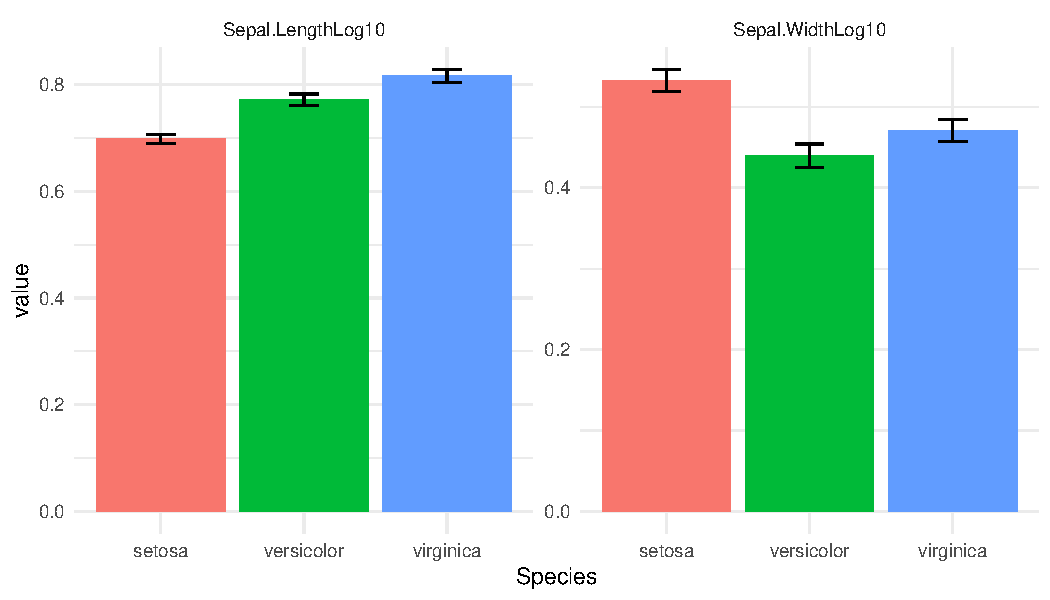
\includegraphics[keepaspectratio]{MANOVA-perMANOVA_files/figure-pdf/fig-manova-means-1.pdf}}

}

\caption{\label{fig-manova-means}Medias (log10) por especie ---
Sepal.LengthLog10 y Sepal.WidthLog10}

\end{figure}%

La Figura~\ref{fig-manova-means} muestra las medias log-transformadas de
las variables \emph{Sepal.Length} y \emph{Sepal.Width} para cada especie
de \emph{iris}, junto con sus intervalos de confianza al 95\%. Se
observan patrones claros y coherentes con los resultados del MANOVA y
las pruebas post-hoc:

\textbf{Sepal.LengthLog10:}\\
Las especies se separan de forma marcada. \emph{Setosa} presenta los
valores más bajos, seguida por \emph{versicolor}, mientras que
\emph{virginica} muestra los sépalos más largos. Los intervalos de
confianza no se superponen, lo que confirma las diferencias
significativas detectadas.

\textbf{Sepal.WidthLog10:}\\
El patrón se invierte parcialmente. \emph{Setosa} posee sépalos más
anchos, mientras que \emph{versicolor} y \emph{virginica} presentan
valores menores. Las diferencias son significativas, aunque de menor
magnitud que en el largo del sépalo.

En conjunto, el gráfico refuerza la evidencia de diferencias
morfológicas consistentes entre las tres especies, evidenciando que las
dimensiones del sépalo son determinantes para su discriminación
multivariada.

\section{perMANOVA}\label{permanova}

\begin{Shaded}
\begin{Highlighting}[numbers=left,,]
\CommentTok{\# perMANOVA: diferencias multivariadas entre especies}

\CommentTok{\# Base de datos (usa df\_manova si ya la tienes del MANOVA)}
\FunctionTok{data}\NormalTok{(}\StringTok{"iris"}\NormalTok{)}
\NormalTok{df\_permanova }\OtherTok{\textless{}{-}}\NormalTok{ df\_manova }\SpecialCharTok{\%\textgreater{}\%}
  \FunctionTok{select}\NormalTok{(Sepal.Length, Sepal.Width, Species)}

\CommentTok{\# Ejecutar perMANOVA (distancia euclidiana)}
\FunctionTok{set.seed}\NormalTok{(}\DecValTok{123}\NormalTok{)}
\NormalTok{permanova\_res }\OtherTok{\textless{}{-}} \FunctionTok{adonis2}\NormalTok{(df\_permanova[,}\DecValTok{1}\SpecialCharTok{:}\DecValTok{2}\NormalTok{] }\SpecialCharTok{\textasciitilde{}}\NormalTok{ Species,}
                         \AttributeTok{data =}\NormalTok{ df\_permanova,}
                         \AttributeTok{method =} \StringTok{"euclidean"}\NormalTok{)}

\CommentTok{\# Convertir a tibble para tabla}
\NormalTok{permanova\_tbl }\OtherTok{\textless{}{-}} \FunctionTok{as\_tibble}\NormalTok{(permanova\_res, }\AttributeTok{rownames =} \StringTok{"Term"}\NormalTok{) }\SpecialCharTok{\%\textgreater{}\%}
  \FunctionTok{mutate}\NormalTok{(}
    \FunctionTok{across}\NormalTok{(}\FunctionTok{where}\NormalTok{(is.numeric), }\SpecialCharTok{\textasciitilde{}} \FunctionTok{round}\NormalTok{(., }\DecValTok{4}\NormalTok{)),}
    \StringTok{\textasciigrave{}}\AttributeTok{Pr(\textgreater{}F)}\StringTok{\textasciigrave{}} \OtherTok{=} \FunctionTok{ifelse}\NormalTok{(}\StringTok{\textasciigrave{}}\AttributeTok{Pr(\textgreater{}F)}\StringTok{\textasciigrave{}} \SpecialCharTok{\textless{}} \FloatTok{0.05}\NormalTok{, }\StringTok{"\textless{} 0.05"}\NormalTok{, }\FunctionTok{round}\NormalTok{(}\StringTok{\textasciigrave{}}\AttributeTok{Pr(\textgreater{}F)}\StringTok{\textasciigrave{}}\NormalTok{, }\DecValTok{4}\NormalTok{))}
\NormalTok{  )}

\NormalTok{knitr}\SpecialCharTok{::}\FunctionTok{kable}\NormalTok{(permanova\_tbl)}
\end{Highlighting}
\end{Shaded}

\begin{longtable}[]{@{}lrrrrl@{}}

\caption{\label{tbl-permanova}Resultado perMANOVA --- modelo:
Sepal.Length + Sepal.Width \textasciitilde{} Species}

\tabularnewline

\toprule\noalign{}
Term & Df & SumOfSqs & R2 & F & Pr(\textgreater F) \\
\midrule\noalign{}
\endhead
\bottomrule\noalign{}
\endlastfoot
Model & 2 & 74.5571 & 0.5714 & 97.9993 & \textless{} 0.05 \\
Residual & 147 & 55.9182 & 0.4286 & NA & NA \\
Total & 149 & 130.4753 & 1.0000 & NA & NA \\

\end{longtable}

La Tabla~\ref{tbl-permanova} presenta los resultados del análisis
perMANOVA, el cual evalúa si existen diferencias multivariadas
significativas en las dimensiones florales (Sepal.Length y Sepal.Width)
entre las especies. El modelo arroja un valor de F ≈ 98 con un p-valor
\textless{} 0.05 , indicando diferencias estadísticamente significativas
entre los grupos.

\begin{Shaded}
\begin{Highlighting}[numbers=left,,]
\CommentTok{\# Función auxiliar que intenta extraer la matriz de p{-}valores de las distintas}
\CommentTok{\# estructuras que puede devolver pairwise.perm.manova()}
\NormalTok{extract\_pairwise\_pvals }\OtherTok{\textless{}{-}} \ControlFlowTok{function}\NormalTok{(obj) \{}
  \CommentTok{\# 1) posibilidad: $P (matriz)}
  \ControlFlowTok{if}\NormalTok{ (}\SpecialCharTok{!}\FunctionTok{is.null}\NormalTok{(obj}\SpecialCharTok{$}\NormalTok{P)) \{}
    \FunctionTok{return}\NormalTok{(}\FunctionTok{as.matrix}\NormalTok{(obj}\SpecialCharTok{$}\NormalTok{P))}
\NormalTok{  \}}
  \CommentTok{\# 2) posibilidad: $Ps}
  \ControlFlowTok{if}\NormalTok{ (}\SpecialCharTok{!}\FunctionTok{is.null}\NormalTok{(obj}\SpecialCharTok{$}\NormalTok{Ps)) \{}
    \FunctionTok{return}\NormalTok{(}\FunctionTok{as.matrix}\NormalTok{(obj}\SpecialCharTok{$}\NormalTok{Ps))}
\NormalTok{  \}}
  \CommentTok{\# 3) posibilidad: $p.value}
  \ControlFlowTok{if}\NormalTok{ (}\SpecialCharTok{!}\FunctionTok{is.null}\NormalTok{(obj}\SpecialCharTok{$}\StringTok{\textasciigrave{}}\AttributeTok{p.value}\StringTok{\textasciigrave{}}\NormalTok{)) \{}
    \FunctionTok{return}\NormalTok{(}\FunctionTok{as.matrix}\NormalTok{(obj}\SpecialCharTok{$}\StringTok{\textasciigrave{}}\AttributeTok{p.value}\StringTok{\textasciigrave{}}\NormalTok{))}
\NormalTok{  \}}
  \CommentTok{\# 4) intentar encontrar la primera matriz numérica en la lista}
\NormalTok{  mats }\OtherTok{\textless{}{-}} \FunctionTok{Filter}\NormalTok{(}\ControlFlowTok{function}\NormalTok{(x) }\FunctionTok{is.matrix}\NormalTok{(x) }\SpecialCharTok{||} \FunctionTok{is.data.frame}\NormalTok{(x), obj)}
  \ControlFlowTok{if}\NormalTok{ (}\FunctionTok{length}\NormalTok{(mats) }\SpecialCharTok{\textgreater{}} \DecValTok{0}\NormalTok{) \{}
\NormalTok{    mm }\OtherTok{\textless{}{-}} \FunctionTok{as.matrix}\NormalTok{(mats[[}\DecValTok{1}\NormalTok{]])}
    \CommentTok{\# si es una matriz triangular con NAs, devolverla}
    \ControlFlowTok{if}\NormalTok{ (}\FunctionTok{is.numeric}\NormalTok{(mm)) }\FunctionTok{return}\NormalTok{(mm)}
\NormalTok{  \}}
  \CommentTok{\# 5) intentar parsear la impresión textual (último recurso)}
  \ControlFlowTok{if}\NormalTok{ (}\SpecialCharTok{!}\FunctionTok{is.null}\NormalTok{(posthoc\_raw\_print) }\SpecialCharTok{\&\&} \FunctionTok{length}\NormalTok{(posthoc\_raw\_print) }\SpecialCharTok{\textgreater{}} \DecValTok{0}\NormalTok{) \{}
    \CommentTok{\# Buscar líneas que parezcan filas de matriz (números con espacios)}
\NormalTok{    lines }\OtherTok{\textless{}{-}}\NormalTok{ posthoc\_raw\_print}
    \CommentTok{\# heurística simple: tomamos las últimas 4 líneas con números}
\NormalTok{    nums\_lines }\OtherTok{\textless{}{-}} \FunctionTok{grep}\NormalTok{(}\StringTok{"}\SpecialCharTok{\textbackslash{}\textbackslash{}}\StringTok{d+}\SpecialCharTok{\textbackslash{}\textbackslash{}}\StringTok{.}\SpecialCharTok{\textbackslash{}\textbackslash{}}\StringTok{d+|\textless{} 0}\SpecialCharTok{\textbackslash{}\textbackslash{}}\StringTok{.0"}\NormalTok{, lines, }\AttributeTok{value =} \ConstantTok{TRUE}\NormalTok{)}
    \ControlFlowTok{if}\NormalTok{ (}\FunctionTok{length}\NormalTok{(nums\_lines) }\SpecialCharTok{\textgreater{}=} \DecValTok{1}\NormalTok{) \{}
      \CommentTok{\# no es perfecto; devolvemos NULL para fallback}
      \FunctionTok{return}\NormalTok{(}\ConstantTok{NULL}\NormalTok{)}
\NormalTok{    \}}
\NormalTok{  \}}
  \FunctionTok{return}\NormalTok{(}\ConstantTok{NULL}\NormalTok{)}
\NormalTok{\}}

\NormalTok{pv\_mat }\OtherTok{\textless{}{-}} \FunctionTok{extract\_pairwise\_pvals}\NormalTok{(posthoc\_permanova)}

\ControlFlowTok{if}\NormalTok{ (}\SpecialCharTok{!}\FunctionTok{is.null}\NormalTok{(pv\_mat)) \{}
  \CommentTok{\# Convertir a tabla larga}
\NormalTok{  ptab }\OtherTok{\textless{}{-}} \FunctionTok{as.data.frame}\NormalTok{(pv\_mat) }\SpecialCharTok{\%\textgreater{}\%}
\NormalTok{    tibble}\SpecialCharTok{::}\FunctionTok{rownames\_to\_column}\NormalTok{(}\StringTok{"Especie1"}\NormalTok{) }\SpecialCharTok{\%\textgreater{}\%}
\NormalTok{    tidyr}\SpecialCharTok{::}\FunctionTok{pivot\_longer}\NormalTok{(}\SpecialCharTok{{-}}\NormalTok{Especie1, }\AttributeTok{names\_to =} \StringTok{"Especie2"}\NormalTok{, }
                        \AttributeTok{values\_to =} \StringTok{"pval"}\NormalTok{) }\SpecialCharTok{\%\textgreater{}\%}
\NormalTok{    dplyr}\SpecialCharTok{::}\FunctionTok{filter}\NormalTok{(}\SpecialCharTok{!}\FunctionTok{is.na}\NormalTok{(pval) }\SpecialCharTok{\&}\NormalTok{ Especie1 }\SpecialCharTok{!=}\NormalTok{ Especie2) }\SpecialCharTok{\%\textgreater{}\%}
\NormalTok{    dplyr}\SpecialCharTok{::}\FunctionTok{mutate}\NormalTok{(}
\NormalTok{      Comparación }\OtherTok{=} \FunctionTok{paste}\NormalTok{(Especie1, Especie2, }\AttributeTok{sep =} \StringTok{" {-} "}\NormalTok{),}
      \AttributeTok{p.value =} \FunctionTok{ifelse}\NormalTok{(}\FunctionTok{as.numeric}\NormalTok{(pval) }\SpecialCharTok{\textless{}} \FloatTok{0.05}\NormalTok{, }\StringTok{"\textless{} 0.05"}\NormalTok{, }
                       \FunctionTok{format}\NormalTok{(}\FunctionTok{round}\NormalTok{(}\FunctionTok{as.numeric}\NormalTok{(pval), }\DecValTok{4}\NormalTok{), }\AttributeTok{nsmall =} \DecValTok{4}\NormalTok{))}
\NormalTok{    ) }\SpecialCharTok{\%\textgreater{}\%}
\NormalTok{    dplyr}\SpecialCharTok{::}\FunctionTok{select}\NormalTok{(Comparación, p.value) }\SpecialCharTok{\%\textgreater{}\%}
\NormalTok{    dplyr}\SpecialCharTok{::}\FunctionTok{distinct}\NormalTok{()}
\NormalTok{\} }\ControlFlowTok{else}\NormalTok{ \{}
\NormalTok{  ptab }\OtherTok{\textless{}{-}} \FunctionTok{tibble}\NormalTok{(}
\NormalTok{    Comparación }\OtherTok{=} \StringTok{"No se pudo extraer la matriz de p{-}valores }
\StringTok{    del objeto devuelto"}\NormalTok{,}
    \AttributeTok{p.value =} \StringTok{"ver output crudo"}
\NormalTok{  )}
\NormalTok{\}}

\NormalTok{knitr}\SpecialCharTok{::}\FunctionTok{kable}\NormalTok{(ptab)}
\end{Highlighting}
\end{Shaded}

\begin{longtable}[]{@{}ll@{}}

\caption{\label{tbl-permanova-posthoc}Comparaciones post-hoc perMANOVA
(ajuste Bonferroni)}

\tabularnewline

\toprule\noalign{}
Comparación & p.value \\
\midrule\noalign{}
\endhead
\bottomrule\noalign{}
\endlastfoot
versicolor - setosa & \textless{} 0.05 \\
virginica - setosa & \textless{} 0.05 \\
virginica - versicolor & \textless{} 0.05 \\

\end{longtable}

La Tabla~\ref{tbl-permanova-posthoc} presenta los resultados de las
comparaciones múltiples post-hoc realizadas tras la perMANOVA. Todas las
comparaciones pareadas entre las especies (\emph{setosa},
\emph{versicolor} y \emph{virginica}) presentan valores \emph{p}
ajustados menores a 0.05, lo que indica diferencias significativas en el
espacio multivariado definido por \emph{Sepal.Length} y
\emph{Sepal.Width}.

\begin{Shaded}
\begin{Highlighting}[numbers=left,,]
\NormalTok{df\_permanova }\SpecialCharTok{\%\textgreater{}\%}
  \FunctionTok{group\_by}\NormalTok{(Species) }\SpecialCharTok{\%\textgreater{}\%}
  \FunctionTok{mutate}\NormalTok{(}\AttributeTok{L =} \FunctionTok{mean}\NormalTok{(Sepal.Length), }\AttributeTok{A =} \FunctionTok{mean}\NormalTok{(Sepal.Width)) }\SpecialCharTok{\%\textgreater{}\%}
  \FunctionTok{ggplot}\NormalTok{(}\FunctionTok{aes}\NormalTok{(Sepal.Length, Sepal.Width, }\AttributeTok{color =}\NormalTok{ Species)) }\SpecialCharTok{+}
  \FunctionTok{geom\_point}\NormalTok{(}\AttributeTok{size =} \DecValTok{2}\NormalTok{, }\AttributeTok{alpha =} \FloatTok{0.8}\NormalTok{) }\SpecialCharTok{+}
  \FunctionTok{geom\_point}\NormalTok{(}\FunctionTok{aes}\NormalTok{(}\AttributeTok{x =}\NormalTok{ L, }\AttributeTok{y =}\NormalTok{ A), }\AttributeTok{size =} \DecValTok{4}\NormalTok{, }\AttributeTok{shape =} \DecValTok{18}\NormalTok{) }\SpecialCharTok{+}
  \FunctionTok{geom\_segment}\NormalTok{(}\FunctionTok{aes}\NormalTok{(}\AttributeTok{xend =}\NormalTok{ L, }\AttributeTok{yend =}\NormalTok{ A), }\AttributeTok{linetype =} \StringTok{"dashed"}\NormalTok{) }\SpecialCharTok{+}
  \FunctionTok{theme\_classic}\NormalTok{() }\SpecialCharTok{+}
  \FunctionTok{labs}\NormalTok{(}\AttributeTok{x =} \StringTok{"Sepal.Length"}\NormalTok{, }\AttributeTok{y =} \StringTok{"Sepal.Width"}\NormalTok{)}
\end{Highlighting}
\end{Shaded}

\begin{figure}[H]

\centering{

\pandocbounded{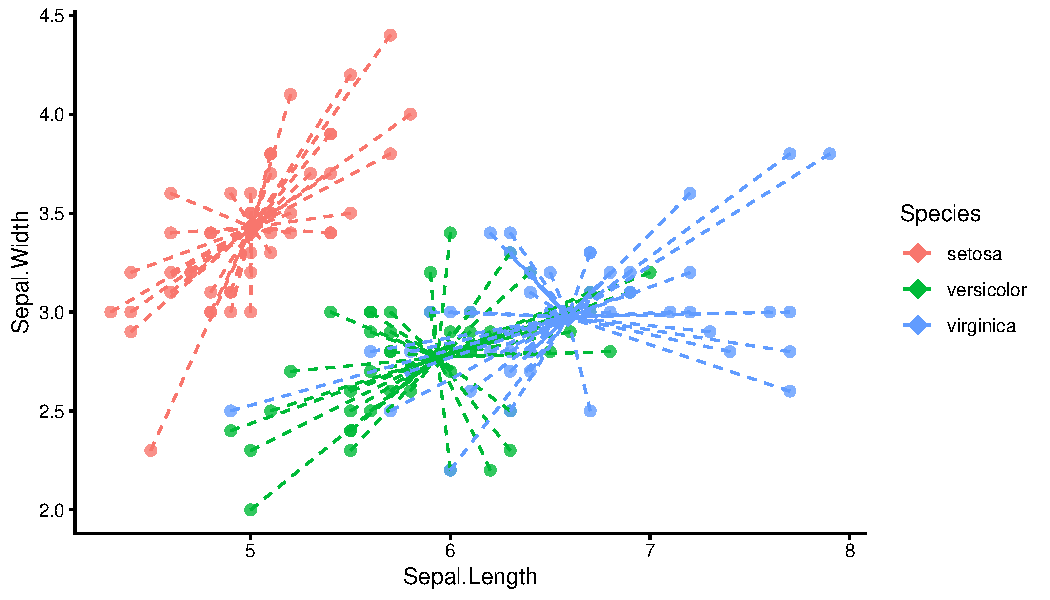
\includegraphics[keepaspectratio]{MANOVA-perMANOVA_files/figure-pdf/fig-permanova-centroides-1.pdf}}

}

\caption{\label{fig-permanova-centroides}Dispersión y centroides por
especie --- Sepal.Length vs Sepal.Width}

\end{figure}%

En la Figura~\ref{fig-permanova-centroides} se aprecia la distribución
de las observaciones de \emph{Sepal.Length} y \emph{Sepal.Width} para
cada especie, junto con sus centroides multivariados. Los tres grupos
presentan una separación clara: \emph{setosa} (rojo) se distingue por
valores de sépalo más cortos y anchos, mientras que \emph{versicolor}
(verde) y \emph{virginica} (azul) muestran mayor longitud y menor ancho,
con cierto solapamiento entre sí. Las líneas discontinuas indican la
dispersión interna de cada especie alrededor de su centroide,
evidenciando una variabilidad relativamente baja dentro de \emph{setosa}
y algo mayor en \emph{versicolor} y \emph{virginica}.

\begin{Shaded}
\begin{Highlighting}[numbers=left,,]
\NormalTok{df\_permanova }\SpecialCharTok{\%\textgreater{}\%}
  \FunctionTok{pivot\_longer}\NormalTok{(}\AttributeTok{cols =} \FunctionTok{c}\NormalTok{(Sepal.Length, Sepal.Width), }
               \AttributeTok{names\_to =} \StringTok{"Variable"}\NormalTok{, }\AttributeTok{values\_to =} \StringTok{"Valor"}\NormalTok{) }\SpecialCharTok{\%\textgreater{}\%}
  \FunctionTok{ggplot}\NormalTok{(}\FunctionTok{aes}\NormalTok{(Variable, Valor, }\AttributeTok{fill =}\NormalTok{ Species)) }\SpecialCharTok{+}
  \FunctionTok{geom\_boxplot}\NormalTok{() }\SpecialCharTok{+}
  \FunctionTok{theme\_classic}\NormalTok{() }\SpecialCharTok{+}
  \FunctionTok{scale\_fill\_brewer}\NormalTok{(}\AttributeTok{palette =} \StringTok{"Set2"}\NormalTok{)}
\end{Highlighting}
\end{Shaded}

\begin{figure}[H]

\centering{

\pandocbounded{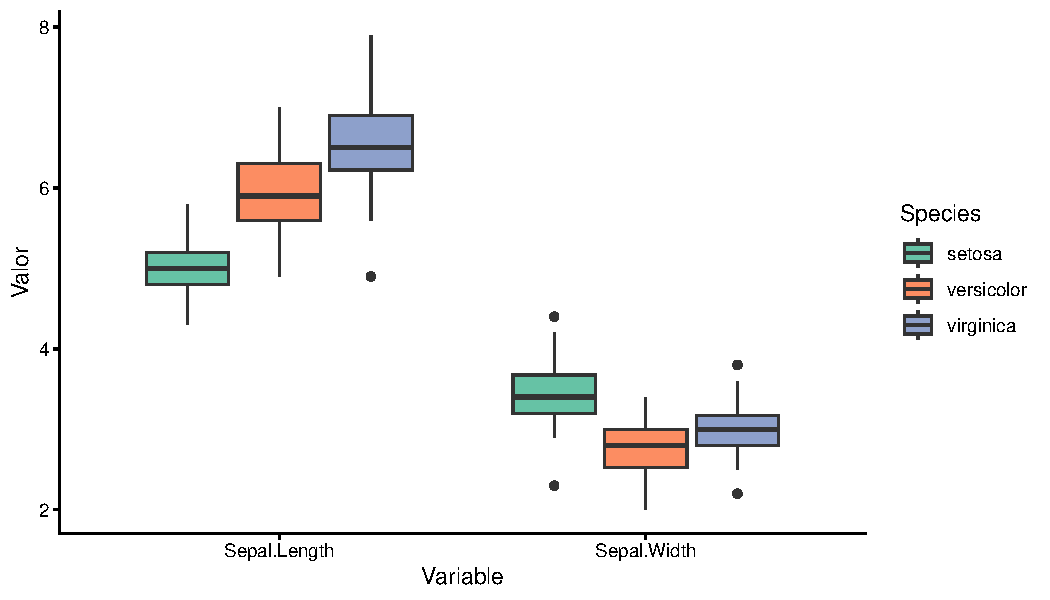
\includegraphics[keepaspectratio]{MANOVA-perMANOVA_files/figure-pdf/fig-permanova-box-1.pdf}}

}

\caption{\label{fig-permanova-box}Distribución por variable y especie
(perMANOVA)}

\end{figure}%

En la Figura~\ref{fig-permanova-box} se representan las distribuciones
de \emph{Sepal.Length} y \emph{Sepal.Width} para cada especie mediante
diagramas de caja. Se observa que \emph{setosa} presenta sépalos
significativamente más cortos pero más anchos en promedio, mientras que
\emph{virginica} muestra los sépalos más largos y angostos;
\emph{versicolor} ocupa una posición intermedia en ambas variables. Las
diferencias entre medianas son notorias y los solapamientos mínimos, lo
que refuerza la existencia de una separación consistente entre especies
en ambas dimensiones morfológicas.

\section{Conclusiones (MANOVA /
perMANOVA)}\label{conclusiones-manova-permanova}

En conjunto, los resultados del MANOVA y del perMANOVA confirman la
existencia de diferencias multivariadas significativas entre las tres
especies de \emph{Iris} en las dimensiones de largo y ancho del sépalo.
El MANOVA basado en los supuestos paramétricos mostró un efecto global
altamente significativo, respaldado por las comparaciones post-hoc y los
gráficos de medias transformadas. A su vez, el perMANOVA una alternativa
no paramétrica más robusta frente a posibles violaciones de los
supuestos replicó el mismo patrón de resultados, detectando diferencias
significativas entre todos los pares de especies. Por lo tanto, los
resultados sustentan la validez de estas variables como criterios
discriminantes entre las especies.




\end{document}
